\documentclass[tikz,border=3pt,multi=tikzpicture]{standalone}
\usepackage{amsmath,amssymb,lmodern}
\usetikzlibrary{arrows.meta,positioning,calc}
\definecolor{Ink}{HTML}{182332}
\definecolor{Blue}{HTML}{245CFF}
\definecolor{Hot}{HTML}{E50078}
\definecolor{Operand}{HTML}{7953C8}
\definecolor{Green}{HTML}{009C73}
\definecolor{Mute}{HTML}{8A96AA}
\newcommand{\sq}{\textcolor{Mute}{\square}}
\newcommand{\focus}[1]{\begingroup\setlength{\fboxsep}{2pt}\setlength{\fboxrule}{0.85pt}\fcolorbox{Hot}{Hot!5}{$\displaystyle #1$}\endgroup}
\tikzset{every node/.style={text=Ink,font=\normalsize},
 box/.style={draw=Blue,line width=.8pt,rounded corners=4pt,inner sep=4pt,fill=Blue!3},
 result/.style={box,draw=Green,fill=Green!3},
 operand/.style={box,draw=Operand,fill=Operand!3},
 lab/.style={font=\sffamily\small,text=Ink!65},
 arrow/.style={-{Stealth[length=4pt]},line width=.9pt,draw=Ink!70}}
\begin{document}
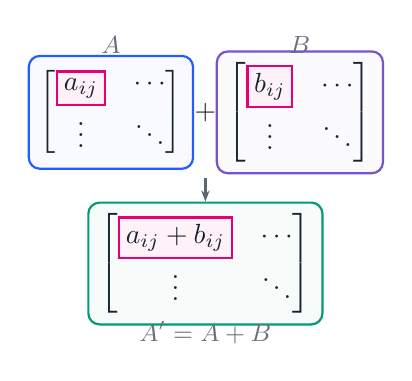
\begin{tikzpicture}
\node[box] (a) at (-1.2,0.8) {$ \begin{bmatrix}\focus{a_{ij}} & \cdots\\\vdots & \ddots\end{bmatrix} $};
\node[operand] (b) at (1.2,0.8) {$ \begin{bmatrix}\focus{b_{ij}} & \cdots\\\vdots & \ddots\end{bmatrix} $};
\node at (0,.8) {$ + $};
\node[lab] at (-1.2,1.65) {$A$};
\node[lab] at (1.2,1.65) {$B$};
\node[result] (c) at (0,-1.12) {$ \begin{bmatrix}\focus{a_{ij}+b_{ij}} & \cdots\\\vdots & \ddots\end{bmatrix} $};
\draw[arrow] (0,-.04) -- (c.north);
\node[lab] at (0,-2) {$A'=A+B$};
\end{tikzpicture}
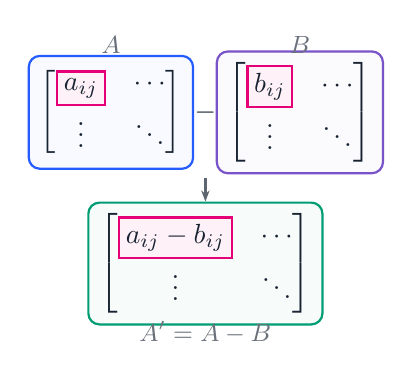
\begin{tikzpicture}
\node[box] (a) at (-1.2,0.8) {$ \begin{bmatrix}\focus{a_{ij}} & \cdots\\\vdots & \ddots\end{bmatrix} $};
\node[operand] (b) at (1.2,0.8) {$ \begin{bmatrix}\focus{b_{ij}} & \cdots\\\vdots & \ddots\end{bmatrix} $};
\node at (0,.8) {$ - $};
\node[lab] at (-1.2,1.65) {$A$};
\node[lab] at (1.2,1.65) {$B$};
\node[result] (c) at (0,-1.12) {$ \begin{bmatrix}\focus{a_{ij}-b_{ij}} & \cdots\\\vdots & \ddots\end{bmatrix} $};
\draw[arrow] (0,-.04) -- (c.north);
\node[lab] at (0,-2) {$A'=A-B$};
\end{tikzpicture}
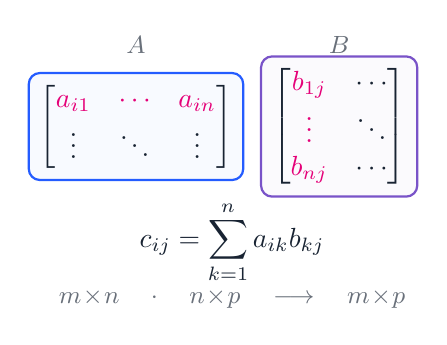
\begin{tikzpicture}
\node[box] (a) at (-1.22,0.25) {$ \begin{bmatrix}\color{Hot}a_{i1} & \color{Hot}\cdots & \color{Hot}a_{in}\\\vdots & \ddots & \vdots\end{bmatrix} $};
\node[operand] (b) at (1.36,0.25) {$ \begin{bmatrix}\color{Hot}b_{1j} & \cdots\\\color{Hot}\vdots & \ddots\\\color{Hot}b_{nj} & \cdots\end{bmatrix} $};
\node[lab] at (-1.22,1.28) {$A$};
\node[lab] at (1.36,1.28) {$B$};
\node at (0,-1.22) {$\displaystyle c_{ij}=\sum_{k=1}^{n} a_{ik}b_{kj}$};
\node[lab] at (0,-1.93) {$m\!\times\!n\quad\cdot\quad n\!\times\!p\quad\longrightarrow\quad m\!\times\!p$};
\end{tikzpicture}
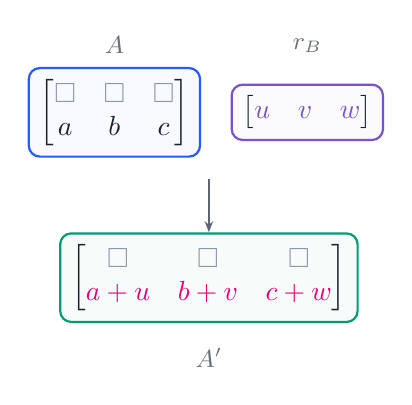
\begin{tikzpicture}
\node[box] (a) at (-1.2,0.8) {$ \begin{bmatrix}\sq & \sq & \sq\\a & b & c\end{bmatrix} $};
\node[operand] (v) at (1.25,0.8) {$ \begin{bmatrix}\color{Operand}u & \color{Operand}v & \color{Operand}w\end{bmatrix} $};
\node[lab] at (-1.2,1.65) {$A$};
\node[lab] at (1.25,1.65) {$r_B$};
\node[result] (b) at (0,-1.3) {$ \begin{bmatrix}\sq & \sq & \sq\\\color{Hot}a+u & \color{Hot}b+v & \color{Hot}c+w\end{bmatrix} $};
\draw[arrow] (0,-.05) -- (b.north);
\node[lab] at (0,-2.32) {$A'$};
\end{tikzpicture}
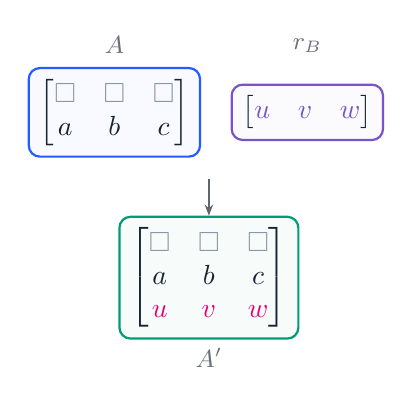
\begin{tikzpicture}
\node[box] (a) at (-1.2,0.8) {$ \begin{bmatrix}\sq & \sq & \sq\\a & b & c\end{bmatrix} $};
\node[operand] (v) at (1.25,0.8) {$ \begin{bmatrix}\color{Operand}u & \color{Operand}v & \color{Operand}w\end{bmatrix} $};
\node[lab] at (-1.2,1.65) {$A$};
\node[lab] at (1.25,1.65) {$r_B$};
\node[result] (b) at (0,-1.3) {$ \begin{bmatrix}\sq & \sq & \sq\\a & b & c\\\color{Hot}u & \color{Hot}v & \color{Hot}w\end{bmatrix} $};
\draw[arrow] (0,-.05) -- (b.north);
\node[lab] at (0,-2.32) {$A'$};
\end{tikzpicture}
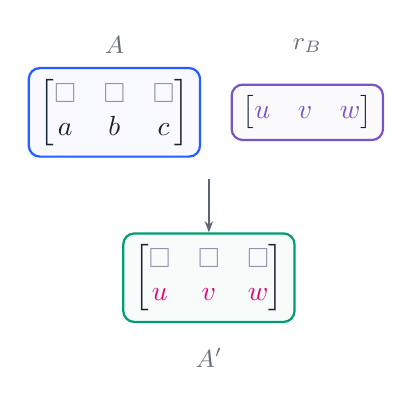
\begin{tikzpicture}
\node[box] (a) at (-1.2,0.8) {$ \begin{bmatrix}\sq & \sq & \sq\\a & b & c\end{bmatrix} $};
\node[operand] (v) at (1.25,0.8) {$ \begin{bmatrix}\color{Operand}u & \color{Operand}v & \color{Operand}w\end{bmatrix} $};
\node[lab] at (-1.2,1.65) {$A$};
\node[lab] at (1.25,1.65) {$r_B$};
\node[result] (b) at (0,-1.3) {$ \begin{bmatrix}\sq & \sq & \sq\\\color{Hot}u & \color{Hot}v & \color{Hot}w\end{bmatrix} $};
\draw[arrow] (0,-.05) -- (b.north);
\node[lab] at (0,-2.32) {$A'$};
\end{tikzpicture}
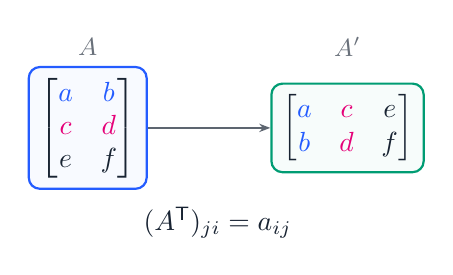
\begin{tikzpicture}
\node[box] (a) at (-1.65,0) {$ \begin{bmatrix}\color{Blue}a & \color{Blue}b\\\color{Hot}c & \color{Hot}d\\e & f\end{bmatrix} $};
\node[result] (b) at (1.65,0) {$ \begin{bmatrix}\color{Blue}a & \color{Hot}c & e\\\color{Blue}b & \color{Hot}d & f\end{bmatrix} $};
\draw[arrow] (a.east) -- (b.west);
\node[lab] at (-1.65,1.03) {$A$};
\node[lab] at (1.65,1.03) {$A'$};
\node at (0,-1.2) {$ (A^{\mathsf T})_{ji}=a_{ij} $};
\end{tikzpicture}
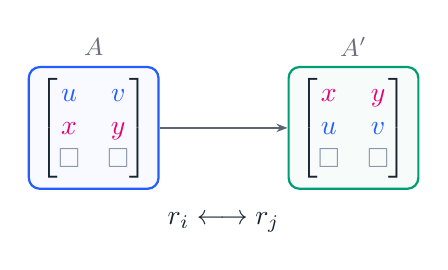
\begin{tikzpicture}
\node[box] (a) at (-1.65,0) {$ \begin{bmatrix}\color{Blue}u & \color{Blue}v\\\color{Hot}x & \color{Hot}y\\\sq & \sq\end{bmatrix} $};
\node[result] (b) at (1.65,0) {$ \begin{bmatrix}\color{Hot}x & \color{Hot}y\\\color{Blue}u & \color{Blue}v\\\sq & \sq\end{bmatrix} $};
\draw[arrow] (a.east) -- (b.west);
\node[lab] at (-1.65,1.03) {$A$};
\node[lab] at (1.65,1.03) {$A'$};
\node at (0,-1.2) {$ r_i\longleftrightarrow r_j $};
\end{tikzpicture}
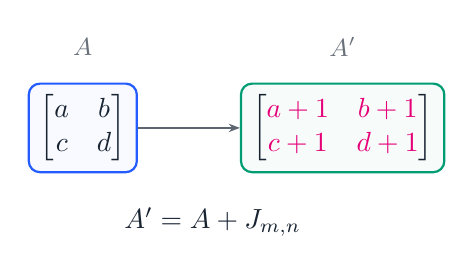
\begin{tikzpicture}
\node[box] (a) at (-1.65,0) {$ \begin{bmatrix}a & b\\c & d\end{bmatrix} $};
\node[result] (b) at (1.65,0) {$ \begin{bmatrix}\color{Hot}a+1 & \color{Hot}b+1\\\color{Hot}c+1 & \color{Hot}d+1\end{bmatrix} $};
\draw[arrow] (a.east) -- (b.west);
\node[lab] at (-1.65,1.03) {$A$};
\node[lab] at (1.65,1.03) {$A'$};
\node at (0,-1.2) {$ A'=A+J_{m,n} $};
\end{tikzpicture}
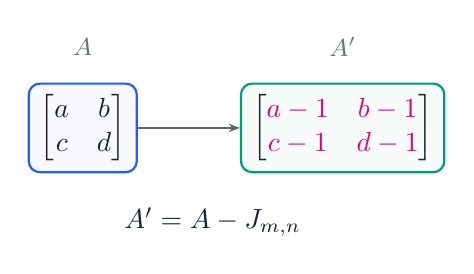
\begin{tikzpicture}
\node[box] (a) at (-1.65,0) {$ \begin{bmatrix}a & b\\c & d\end{bmatrix} $};
\node[result] (b) at (1.65,0) {$ \begin{bmatrix}\color{Hot}a-1 & \color{Hot}b-1\\\color{Hot}c-1 & \color{Hot}d-1\end{bmatrix} $};
\draw[arrow] (a.east) -- (b.west);
\node[lab] at (-1.65,1.03) {$A$};
\node[lab] at (1.65,1.03) {$A'$};
\node at (0,-1.2) {$ A'=A-J_{m,n} $};
\end{tikzpicture}
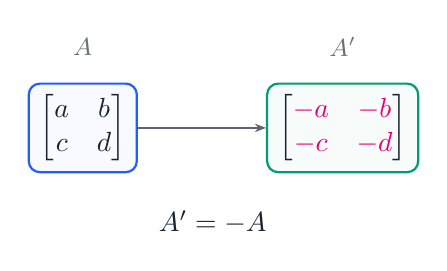
\begin{tikzpicture}
\node[box] (a) at (-1.65,0) {$ \begin{bmatrix}a & b\\c & d\end{bmatrix} $};
\node[result] (b) at (1.65,0) {$ \begin{bmatrix}\color{Hot}-a & \color{Hot}-b\\\color{Hot}-c & \color{Hot}-d\end{bmatrix} $};
\draw[arrow] (a.east) -- (b.west);
\node[lab] at (-1.65,1.03) {$A$};
\node[lab] at (1.65,1.03) {$A'$};
\node at (0,-1.2) {$ A'=-A $};
\end{tikzpicture}
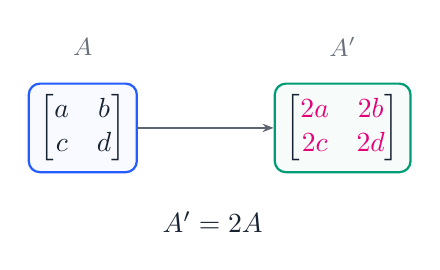
\begin{tikzpicture}
\node[box] (a) at (-1.65,0) {$ \begin{bmatrix}a & b\\c & d\end{bmatrix} $};
\node[result] (b) at (1.65,0) {$ \begin{bmatrix}\color{Hot}2a & \color{Hot}2b\\\color{Hot}2c & \color{Hot}2d\end{bmatrix} $};
\draw[arrow] (a.east) -- (b.west);
\node[lab] at (-1.65,1.03) {$A$};
\node[lab] at (1.65,1.03) {$A'$};
\node at (0,-1.2) {$ A'=2A $};
\end{tikzpicture}
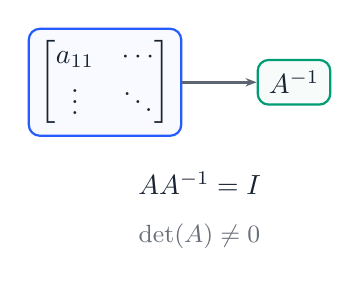
\begin{tikzpicture}
\node[box] (a) at (-1.2,0.2) {$ \begin{bmatrix}a_{11} & \cdots\\\vdots & \ddots\end{bmatrix} $};
\node[result] (b) at (1.2,0.2) {$ A^{-1} $};
\draw[arrow] (a.east) -- (b.west);
\node at (0,-1.08) {$AA^{-1}=I$};
\node[lab] at (0,-1.75) {$\det(A)\ne0$};
\end{tikzpicture}
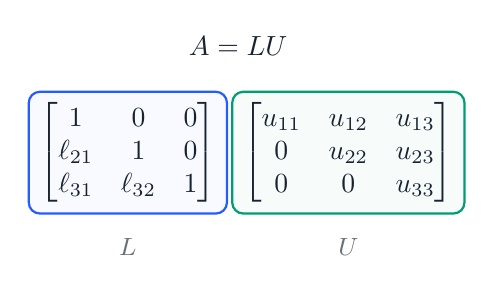
\begin{tikzpicture}
\node at (0,1.35) {$A=LU$};
\node[box] (l) at (-1.4,0) {$ \begin{bmatrix}1 & 0 & 0\\\ell_{21} & 1 & 0\\\ell_{31} & \ell_{32} & 1\end{bmatrix} $};
\node[result] (u) at (1.4,0) {$ \begin{bmatrix}u_{11} & u_{12} & u_{13}\\0 & u_{22} & u_{23}\\0 & 0 & u_{33}\end{bmatrix} $};
\node[lab] at (-1.4,-1.2) {$L$};
\node[lab] at (1.4,-1.2) {$U$};
\end{tikzpicture}
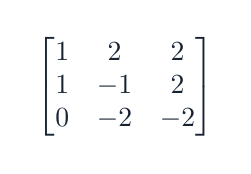
\begin{tikzpicture}
\node at (0,0) {$\displaystyle \begin{bmatrix}1 & 2 & 2\\1 & -1 & 2\\0 & -2 & -2\end{bmatrix}$};
\end{tikzpicture}
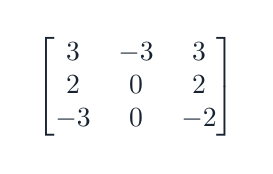
\begin{tikzpicture}
\node at (0,0) {$\displaystyle \begin{bmatrix}3 & -3 & 3\\2 & 0 & 2\\-3 & 0 & -2\end{bmatrix}$};
\end{tikzpicture}
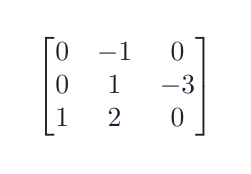
\begin{tikzpicture}
\node at (0,0) {$\displaystyle \begin{bmatrix}0 & -1 & 0\\0 & 1 & -3\\1 & 2 & 0\end{bmatrix}$};
\end{tikzpicture}
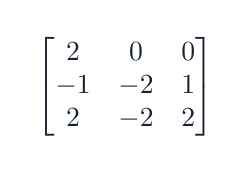
\begin{tikzpicture}
\node at (0,0) {$\displaystyle \begin{bmatrix}2 & 0 & 0\\-1 & -2 & 1\\2 & -2 & 2\end{bmatrix}$};
\end{tikzpicture}
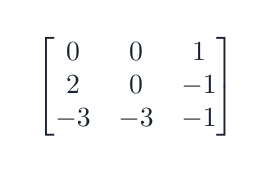
\begin{tikzpicture}
\node at (0,0) {$\displaystyle \begin{bmatrix}0 & 0 & 1\\2 & 0 & -1\\-3 & -3 & -1\end{bmatrix}$};
\end{tikzpicture}
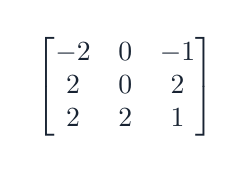
\begin{tikzpicture}
\node at (0,0) {$\displaystyle \begin{bmatrix}-2 & 0 & -1\\2 & 0 & 2\\2 & 2 & 1\end{bmatrix}$};
\end{tikzpicture}
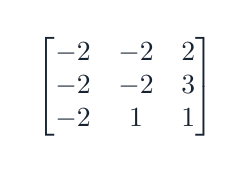
\begin{tikzpicture}
\node at (0,0) {$\displaystyle \begin{bmatrix}-2 & -2 & 2\\-2 & -2 & 3\\-2 & 1 & 1\end{bmatrix}$};
\end{tikzpicture}
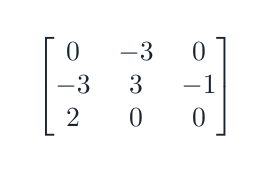
\begin{tikzpicture}
\node at (0,0) {$\displaystyle \begin{bmatrix}0 & -3 & 0\\-3 & 3 & -1\\2 & 0 & 0\end{bmatrix}$};
\end{tikzpicture}
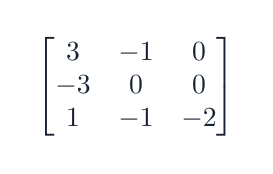
\begin{tikzpicture}
\node at (0,0) {$\displaystyle \begin{bmatrix}3 & -1 & 0\\-3 & 0 & 0\\1 & -1 & -2\end{bmatrix}$};
\end{tikzpicture}
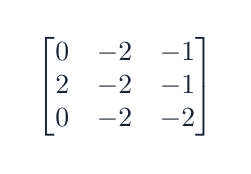
\begin{tikzpicture}
\node at (0,0) {$\displaystyle \begin{bmatrix}0 & -2 & -1\\2 & -2 & -1\\0 & -2 & -2\end{bmatrix}$};
\end{tikzpicture}
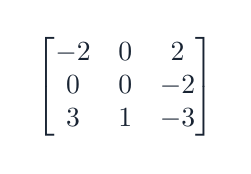
\begin{tikzpicture}
\node at (0,0) {$\displaystyle \begin{bmatrix}-2 & 0 & 2\\0 & 0 & -2\\3 & 1 & -3\end{bmatrix}$};
\end{tikzpicture}
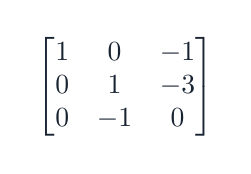
\begin{tikzpicture}
\node at (0,0) {$\displaystyle \begin{bmatrix}1 & 0 & -1\\0 & 1 & -3\\0 & -1 & 0\end{bmatrix}$};
\end{tikzpicture}
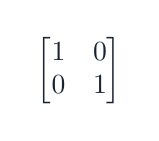
\begin{tikzpicture}
\node at (0,0) {$\displaystyle \begin{bmatrix}1 & 0\\0 & 1\end{bmatrix}$};
\end{tikzpicture}
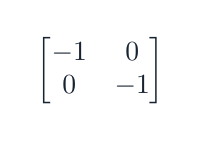
\begin{tikzpicture}
\node at (0,0) {$\displaystyle \begin{bmatrix}-1 & 0\\0 & -1\end{bmatrix}$};
\end{tikzpicture}
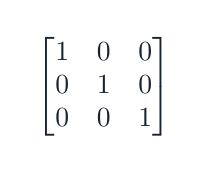
\begin{tikzpicture}
\node at (0,0) {$\displaystyle \begin{bmatrix}1 & 0 & 0\\0 & 1 & 0\\0 & 0 & 1\end{bmatrix}$};
\end{tikzpicture}
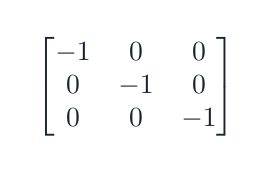
\begin{tikzpicture}
\node at (0,0) {$\displaystyle \begin{bmatrix}-1 & 0 & 0\\0 & -1 & 0\\0 & 0 & -1\end{bmatrix}$};
\end{tikzpicture}
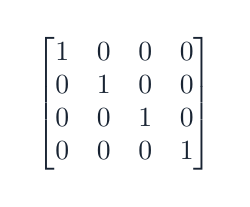
\begin{tikzpicture}
\node at (0,0) {$\displaystyle \begin{bmatrix}1 & 0 & 0 & 0\\0 & 1 & 0 & 0\\0 & 0 & 1 & 0\\0 & 0 & 0 & 1\end{bmatrix}$};
\end{tikzpicture}
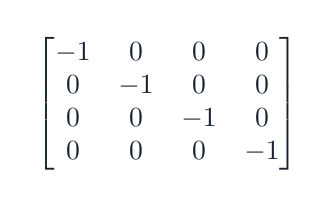
\begin{tikzpicture}
\node at (0,0) {$\displaystyle \begin{bmatrix}-1 & 0 & 0 & 0\\0 & -1 & 0 & 0\\0 & 0 & -1 & 0\\0 & 0 & 0 & -1\end{bmatrix}$};
\end{tikzpicture}
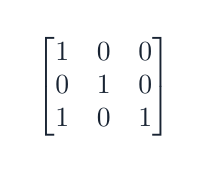
\begin{tikzpicture}
\node at (0,0) {$\displaystyle \begin{bmatrix}1 & 0 & 0\\0 & 1 & 0\\1 & 0 & 1\end{bmatrix}$};
\end{tikzpicture}
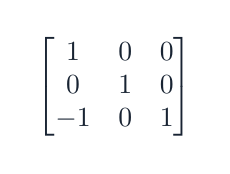
\begin{tikzpicture}
\node at (0,0) {$\displaystyle \begin{bmatrix}1 & 0 & 0\\0 & 1 & 0\\-1 & 0 & 1\end{bmatrix}$};
\end{tikzpicture}
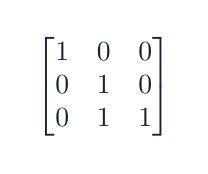
\begin{tikzpicture}
\node at (0,0) {$\displaystyle \begin{bmatrix}1 & 0 & 0\\0 & 1 & 0\\0 & 1 & 1\end{bmatrix}$};
\end{tikzpicture}
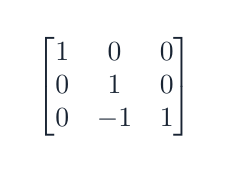
\begin{tikzpicture}
\node at (0,0) {$\displaystyle \begin{bmatrix}1 & 0 & 0\\0 & 1 & 0\\0 & -1 & 1\end{bmatrix}$};
\end{tikzpicture}
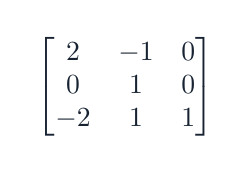
\begin{tikzpicture}
\node at (0,0) {$\displaystyle \begin{bmatrix}2 & -1 & 0\\0 & 1 & 0\\-2 & 1 & 1\end{bmatrix}$};
\end{tikzpicture}
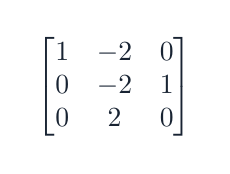
\begin{tikzpicture}
\node at (0,0) {$\displaystyle \begin{bmatrix}1 & -2 & 0\\0 & -2 & 1\\0 & 2 & 0\end{bmatrix}$};
\end{tikzpicture}
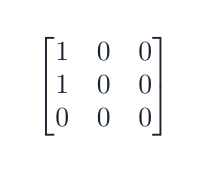
\begin{tikzpicture}
\node at (0,0) {$\displaystyle \begin{bmatrix}1 & 0 & 0\\1 & 0 & 0\\0 & 0 & 0\end{bmatrix}$};
\end{tikzpicture}
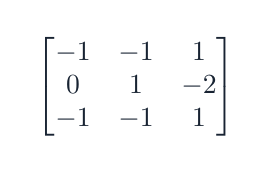
\begin{tikzpicture}
\node at (0,0) {$\displaystyle \begin{bmatrix}-1 & -1 & 1\\0 & 1 & -2\\-1 & -1 & 1\end{bmatrix}$};
\end{tikzpicture}
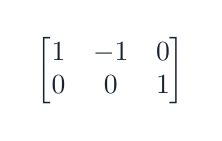
\begin{tikzpicture}
\node at (0,0) {$\displaystyle \begin{bmatrix}1 & -1 & 0\\0 & 0 & 1\end{bmatrix}$};
\end{tikzpicture}
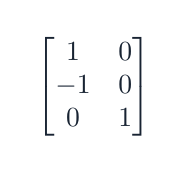
\begin{tikzpicture}
\node at (0,0) {$\displaystyle \begin{bmatrix}1 & 0\\-1 & 0\\0 & 1\end{bmatrix}$};
\end{tikzpicture}
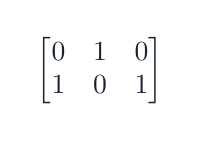
\begin{tikzpicture}
\node at (0,0) {$\displaystyle \begin{bmatrix}0 & 1 & 0\\1 & 0 & 1\end{bmatrix}$};
\end{tikzpicture}
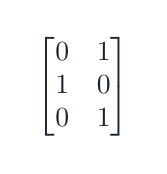
\begin{tikzpicture}
\node at (0,0) {$\displaystyle \begin{bmatrix}0 & 1\\1 & 0\\0 & 1\end{bmatrix}$};
\end{tikzpicture}
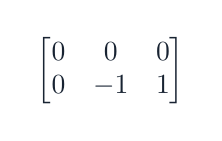
\begin{tikzpicture}
\node at (0,0) {$\displaystyle \begin{bmatrix}0 & 0 & 0\\0 & -1 & 1\end{bmatrix}$};
\end{tikzpicture}
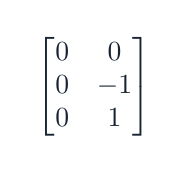
\begin{tikzpicture}
\node at (0,0) {$\displaystyle \begin{bmatrix}0 & 0\\0 & -1\\0 & 1\end{bmatrix}$};
\end{tikzpicture}
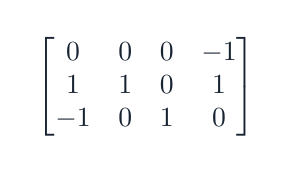
\begin{tikzpicture}
\node at (0,0) {$\displaystyle \begin{bmatrix}0 & 0 & 0 & -1\\1 & 1 & 0 & 1\\-1 & 0 & 1 & 0\end{bmatrix}$};
\end{tikzpicture}
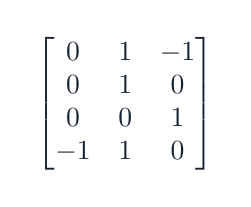
\begin{tikzpicture}
\node at (0,0) {$\displaystyle \begin{bmatrix}0 & 1 & -1\\0 & 1 & 0\\0 & 0 & 1\\-1 & 1 & 0\end{bmatrix}$};
\end{tikzpicture}
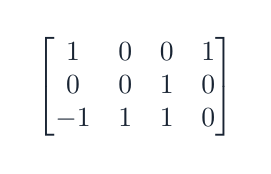
\begin{tikzpicture}
\node at (0,0) {$\displaystyle \begin{bmatrix}1 & 0 & 0 & 1\\0 & 0 & 1 & 0\\-1 & 1 & 1 & 0\end{bmatrix}$};
\end{tikzpicture}
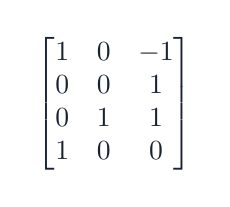
\begin{tikzpicture}
\node at (0,0) {$\displaystyle \begin{bmatrix}1 & 0 & -1\\0 & 0 & 1\\0 & 1 & 1\\1 & 0 & 0\end{bmatrix}$};
\end{tikzpicture}
\begin{tikzpicture}
\node at (0,0) {$\displaystyle \begin{bmatrix}1 & 1 & 0 & 0\\-1 & -2 & 0 & -1\\-1 & 0 & 0 & 1\end{bmatrix}$};
\end{tikzpicture}
\begin{tikzpicture}
\node at (0,0) {$\displaystyle \begin{bmatrix}1 & -1 & -1\\1 & -2 & 0\\0 & 0 & 0\\0 & -1 & 1\end{bmatrix}$};
\end{tikzpicture}
\begin{tikzpicture}
\node at (0,0) {$\displaystyle \begin{bmatrix}0 & 1 & 0 & 1\\1 & -1 & 0 & -2\end{bmatrix}$};
\end{tikzpicture}
\begin{tikzpicture}
\node at (0,0) {$\displaystyle \begin{bmatrix}0 & 1\\1 & -1\\0 & 0\\1 & -2\end{bmatrix}$};
\end{tikzpicture}
\begin{tikzpicture}
\node at (0,0) {$\displaystyle \begin{bmatrix}1 & 1 & 1 & -1\\-1 & -1 & -1 & 1\end{bmatrix}$};
\end{tikzpicture}
\begin{tikzpicture}
\node at (0,0) {$\displaystyle \begin{bmatrix}1 & -1\\1 & -1\\1 & -1\\-1 & 1\end{bmatrix}$};
\end{tikzpicture}
\begin{tikzpicture}
\node at (0,0) {$\displaystyle A^{\mathsf T}=A\qquad\det(A)\ne0$};
\end{tikzpicture}
\begin{tikzpicture}
\node at (0,0) {$\displaystyle \begin{bmatrix}1 & 1 & 0\\1 & 1 & 1\\0 & 1 & 1\end{bmatrix}$};
\end{tikzpicture}
\begin{tikzpicture}
\node at (0,0) {$\displaystyle A=I_n$};
\end{tikzpicture}
\begin{tikzpicture}
\node at (0,0) {$\displaystyle A=-I_n$};
\end{tikzpicture}
\begin{tikzpicture}
\node at (0,0) {$\displaystyle A=\operatorname{diag}(d_1,\ldots,d_n)$};
\end{tikzpicture}
\begin{tikzpicture}
\node at (0,0) {$\displaystyle \begin{bmatrix}1 & 0 & 0\\0 & 2 & 0\\0 & 0 & 3\end{bmatrix}$};
\end{tikzpicture}
\begin{tikzpicture}
\node at (0,0) {$\displaystyle A\mathbf{1}=\mathbf{1}\qquad A^{\mathsf T}\mathbf{1}=\mathbf{1}$};
\end{tikzpicture}
\begin{tikzpicture}
\node at (0,0) {$\displaystyle \begin{bmatrix}1 & 1 & -1\\-1 & 1 & 1\\1 & -1 & 1\end{bmatrix}$};
\end{tikzpicture}
\begin{tikzpicture}
\node at (0,0) {$\displaystyle A^{\mathsf T}=-A\qquad A\ne0$};
\end{tikzpicture}
\begin{tikzpicture}
\node at (0,0) {$\displaystyle \begin{bmatrix}0 & 1 & -1\\-1 & 0 & 1\\1 & -1 & 0\end{bmatrix}$};
\end{tikzpicture}
\begin{tikzpicture}
\node at (0,0) {$\displaystyle A^2=I_n$};
\end{tikzpicture}
\begin{tikzpicture}
\node at (0,0) {$\displaystyle \begin{bmatrix}1 & 1 & 0\\0 & -1 & 0\\0 & 0 & 1\end{bmatrix}$};
\end{tikzpicture}
\begin{tikzpicture}
\node at (0,0) {$\displaystyle \det(A)=1$};
\end{tikzpicture}
\begin{tikzpicture}
\node at (0,0) {$\displaystyle \begin{bmatrix}1 & 1 & 0\\0 & 1 & 1\\1 & 1 & 1\end{bmatrix}$};
\end{tikzpicture}
\begin{tikzpicture}
\node at (0,0) {$\displaystyle A^2=A\qquad\operatorname{rank}(A)=2$};
\end{tikzpicture}
\begin{tikzpicture}
\node at (0,0) {$\displaystyle \begin{bmatrix}1 & 1 & 0\\0 & 0 & 0\\0 & 0 & 1\end{bmatrix}$};
\end{tikzpicture}
\begin{tikzpicture}
\node at (0,0) {$\displaystyle A^3=0\qquad A^2\ne0$};
\end{tikzpicture}
\begin{tikzpicture}
\node at (0,0) {$\displaystyle \begin{bmatrix}0 & 1 & 0\\0 & 0 & 1\\0 & 0 & 0\end{bmatrix}$};
\end{tikzpicture}
\begin{tikzpicture}
\node at (0,0) {$\displaystyle A^3=I_n$};
\end{tikzpicture}
\begin{tikzpicture}
\node at (0,0) {$\displaystyle \begin{bmatrix}0 & 1 & 1\\0 & 0 & 1\\1 & -1 & 0\end{bmatrix}$};
\end{tikzpicture}
\begin{tikzpicture}
\node at (0,0) {$\displaystyle \begin{gathered}A^{\mathsf T}A=D\\D=\operatorname{diag}(d_1,\ldots,d_n),\quad d_i>0\end{gathered}$};
\end{tikzpicture}
\begin{tikzpicture}
\node at (0,0) {$\displaystyle \begin{bmatrix}1 & 1\\1 & -1\\1 & 0\end{bmatrix}$};
\end{tikzpicture}
\begin{tikzpicture}
\node at (0,0) {$\displaystyle \begin{gathered}AA^{\mathsf T}=D\\D=\operatorname{diag}(d_1,\ldots,d_m),\quad d_i>0\end{gathered}$};
\end{tikzpicture}
\begin{tikzpicture}
\node at (0,0) {$\displaystyle \begin{bmatrix}1 & 1 & 1\\1 & -1 & 0\end{bmatrix}$};
\end{tikzpicture}
\begin{tikzpicture}
\node at (0,0) {$\displaystyle A\mathbf{1}=n\mathbf{1}\qquad A^{\mathsf T}\mathbf{1}=m\mathbf{1}$};
\end{tikzpicture}
\begin{tikzpicture}
\node at (0,0) {$\displaystyle \begin{bmatrix}-1 & 3 & 1\\3 & -1 & 1\end{bmatrix}$};
\end{tikzpicture}
\begin{tikzpicture}
\node at (0,0) {$\displaystyle \begin{gathered}A\mathbf{1}=0\\AA^{\mathsf T}=\operatorname{diag}(d_i),\quad d_i>0\end{gathered}$};
\end{tikzpicture}
\begin{tikzpicture}
\node at (0,0) {$\displaystyle \begin{bmatrix}1 & -1 & 0\\1 & 1 & -2\end{bmatrix}$};
\end{tikzpicture}
\begin{tikzpicture}
\node[box] (a) at (-1.65,0) {$ \begin{bmatrix}\sq & \sq & \sq\\\sq & \focus{x} & \sq\\\sq & \sq & \sq\end{bmatrix} $};
\node[result] (b) at (1.65,0) {$ \begin{bmatrix}\sq & \sq & \sq\\\sq & \focus{x\pm1} & \sq\\\sq & \sq & \sq\end{bmatrix} $};
\draw[arrow] (a.east) -- (b.west);
\node[lab] at (-1.65,1.03) {$A$};
\node[lab] at (1.65,1.03) {$A'$};
\node at (0,-1.2) {$ a'_{ij}=x\pm1 $};
\end{tikzpicture}
\begin{tikzpicture}
\node[box] (a) at (-1.65,0) {$ \begin{bmatrix}\sq & \sq & \sq\\\sq & \focus{x} & \sq\\\sq & \sq & \sq\end{bmatrix} $};
\node[result] (b) at (1.65,0) {$ \begin{bmatrix}\sq & \sq & \sq\\\sq & \focus{0} & \sq\\\sq & \sq & \sq\end{bmatrix} $};
\draw[arrow] (a.east) -- (b.west);
\node[lab] at (-1.65,1.03) {$A$};
\node[lab] at (1.65,1.03) {$A'$};
\node at (0,-1.2) {$ a'_{ij}=0 $};
\end{tikzpicture}
\begin{tikzpicture}
\node[box] (a) at (-1.65,0) {$ \begin{bmatrix}\color{Blue}u & \color{Blue}v\\\color{Hot}a & \color{Hot}b\\\sq & \sq\end{bmatrix} $};
\node[result] (b) at (1.65,0) {$ \begin{bmatrix}\color{Blue}u & \color{Blue}v\\\color{Hot}a\pm u & \color{Hot}b\pm v\\\sq & \sq\end{bmatrix} $};
\draw[arrow] (a.east) -- (b.west);
\node[lab] at (-1.65,1.03) {$A$};
\node[lab] at (1.65,1.03) {$A'$};
\node at (0,-1.2) {$ r_j'=r_j\pm r_i,\qquad i\ne j $};
\end{tikzpicture}
\begin{tikzpicture}
\node[box] (a) at (-1.65,0) {$ \begin{bmatrix}\sq & \sq & \sq\\\sq & \focus{x} & \sq\\\sq & \sq & \sq\end{bmatrix} $};
\node[result] (b) at (1.65,0) {$ \begin{bmatrix}\sq & \sq & \sq\\\sq & \focus{x+1} & \sq\\\sq & \sq & \sq\end{bmatrix} $};
\draw[arrow] (a.east) -- (b.west);
\node[lab] at (-1.65,1.03) {$A$};
\node[lab] at (1.65,1.03) {$A'$};
\node at (0,-1.2) {$ a'_{ij}=x+1 $};
\end{tikzpicture}
\begin{tikzpicture}
\node[box] (a) at (-1.65,0) {$ \begin{bmatrix}\sq & \sq & \sq\\\sq & \focus{x} & \sq\\\sq & \sq & \sq\end{bmatrix} $};
\node[result] (b) at (1.65,0) {$ \begin{bmatrix}\sq & \sq & \sq\\\sq & \focus{x-1} & \sq\\\sq & \sq & \sq\end{bmatrix} $};
\draw[arrow] (a.east) -- (b.west);
\node[lab] at (-1.65,1.03) {$A$};
\node[lab] at (1.65,1.03) {$A'$};
\node at (0,-1.2) {$ a'_{ij}=x-1 $};
\end{tikzpicture}
\end{document}
